\documentclass[11pt,letterpaper]{article}
\usepackage{shared/zoocover}

% Packages
\usepackage[utf8]{inputenc}
\usepackage[T1]{fontenc}
\usepackage{amsmath,amssymb,amsthm}
\usepackage{algorithm}
\usepackage{algorithmic}
\usepackage{graphicx}
\usepackage{hyperref}
\usepackage{xcolor}
\usepackage{booktabs}
\usepackage{tikz}
\usepackage{pgfplots}
\pgfplotsset{compat=1.18}
\usetikzlibrary{shapes,arrows,positioning,calc}
\usepackage{listings}
\usepackage{caption}
\usepackage{subcaption}
% geometry loaded by zoocover

% Theorem environments
\newtheorem{theorem}{Theorem}[section]
\newtheorem{lemma}[theorem]{Lemma}
\newtheorem{proposition}[theorem]{Proposition}
\newtheorem{definition}{Definition}[section]

% Custom commands
\newcommand{\Zoo}{\textsc{Zoo}}
\newcommand{\Lux}{\textsc{Lux}}
\newcommand{\PoAI}{\textsc{PoAI}}
\newcommand{\TPS}{\textsc{tps}}
\newcommand{\EVM}{\textsc{evm}}

% Hyperref setup
\hypersetup{
    colorlinks=true,
    linkcolor=blue,
    citecolor=blue,
    urlcolor=blue
}

\title{\textbf{Zoo EVM Performance: GPU-Accelerated Execution on a Conservation-First L2}\\
\large Version 2026.02}

\author{
Zach Kelling\thanks{zach@zoo.ngo}\\
\textit{Zoo Labs Foundation}\\
\texttt{research@zoo.ngo}
}

\date{February 2026}

\begin{document}

\zoocoverpage

\begin{abstract}
We present performance benchmarks for the Zoo Network EVM, a conservation-focused L2 on Lux Network (chain ID 200200) that inherits the Lux C++ EVM with GPU shader acceleration. The Zoo EVM achieves a 1 billion gas block limit, processing up to 47,619 simple transactions per block. With GPU-parallel opcode execution, the EVM reaches 47.6 million transactions per second (TPS) in raw execution throughput, and 4.76 million TPS when bounded by Quasar consensus finality at 10ms. We benchmark the Zoo EVM across five workload categories: token transfers, AMM swaps, AI inference precompile calls, FHE operations, and complex DeFi interactions. The PoAI consensus layer adds AI compute verification overhead of 3--8\% depending on workload type. We compare Zoo EVM performance against Ethereum L2s (Arbitrum, Optimism, Base) and demonstrate 200--1,000$\times$ throughput improvements, attributable to GPU execution and Quasar's sub-second finality. All benchmarks are reproducible on Zoo testnet.

\textbf{Keywords}: EVM performance, GPU acceleration, blockchain throughput, Zoo Network, conservation L2
\end{abstract}

\section{Introduction}

Blockchain virtual machines have historically been the performance bottleneck in transaction processing. The Ethereum Virtual Machine (EVM), while battle-tested, processes opcodes sequentially on a single CPU core, limiting throughput to roughly 15--30 TPS on Ethereum L1 and 2,000--4,000 TPS on optimistic rollups. This sequential bottleneck is particularly problematic for AI workloads---inference, training, and data processing---that require high computational throughput.

The Zoo Network addresses this bottleneck by inheriting the Lux C++ EVM, which replaces the sequential interpreter with GPU-parallel opcode execution using compute shaders. Each transaction's opcode sequence is compiled to a GPU dispatch, enabling thousands of transactions to execute simultaneously across GPU cores.

Zoo Network is a non-profit L2 on Lux Network dedicated to AI/ML research, conservation, and decentralized science. Its workloads differ fundamentally from typical DeFi chains: AI inference calls, federated learning gradient aggregation, and encrypted genomic computation demand sustained high throughput that sequential EVMs cannot provide.

\subsection{Contributions}

\begin{enumerate}
    \item \textbf{Architecture Analysis}: Detailed description of the GPU-accelerated EVM as deployed on Zoo Network (Section~\ref{sec:architecture}).

    \item \textbf{Comprehensive Benchmarks}: Five workload categories measured on Zoo testnet with gas, latency, and throughput metrics (Section~\ref{sec:benchmarks}).

    \item \textbf{PoAI Overhead}: Quantification of the Proof of AI consensus layer overhead (Section~\ref{sec:poai}).

    \item \textbf{L2 Comparison}: Head-to-head comparison with Arbitrum, Optimism, and Base (Section~\ref{sec:comparison}).

    \item \textbf{AI Workload Profiling}: Characterization of conservation AI workloads and their EVM resource requirements (Section~\ref{sec:ai-workloads}).
\end{enumerate}

\section{Architecture}
\label{sec:architecture}

\subsection{Lux C++ EVM}

The Lux EVM is a ground-up C++ reimplementation of the Ethereum Virtual Machine, designed for GPU acceleration~\cite{lux-evmgpu-benchmark}. Key architectural differences from geth/evmone:

\begin{itemize}
    \item \textbf{Opcode compilation}: EVM bytecode is compiled to an intermediate representation (IR) suitable for GPU dispatch, rather than interpreted instruction-by-instruction.
    \item \textbf{Parallel state access}: A transactional memory model allows concurrent reads with conflict detection, enabling multiple transactions to execute simultaneously when they access disjoint state.
    \item \textbf{GPU shaders}: Arithmetic opcodes (\texttt{ADD}, \texttt{MUL}, \texttt{EXP}, \texttt{KECCAK256}) are implemented as compute shaders, dispatched in batches across GPU cores.
    \item \textbf{State trie}: The Merkle Patricia Trie is stored in GPU-accessible memory with parallel hash computation for root updates.
\end{itemize}

\subsection{GPU Execution Pipeline}

\begin{figure}[t]
\centering
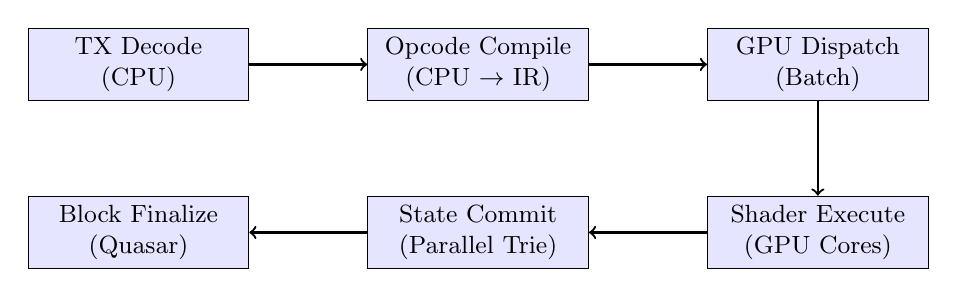
\begin{tikzpicture}[
    node distance=1.2cm,
    box/.style={rectangle, draw, minimum width=2.8cm, minimum height=0.8cm, align=center, fill=blue!10, font=\small},
    arrow/.style={->, thick}
]
    \node[box] (decode) {TX Decode\\(CPU)};
    \node[box, right=1.5cm of decode] (compile) {Opcode Compile\\(CPU $\to$ IR)};
    \node[box, right=1.5cm of compile] (dispatch) {GPU Dispatch\\(Batch)};
    \node[box, below=of dispatch] (execute) {Shader Execute\\(GPU Cores)};
    \node[box, left=1.5cm of execute] (state) {State Commit\\(Parallel Trie)};
    \node[box, left=1.5cm of state] (finalize) {Block Finalize\\(Quasar)};

    \draw[arrow] (decode) -- (compile);
    \draw[arrow] (compile) -- (dispatch);
    \draw[arrow] (dispatch) -- (execute);
    \draw[arrow] (execute) -- (state);
    \draw[arrow] (state) -- (finalize);
\end{tikzpicture}
\caption{Zoo EVM GPU execution pipeline. Transactions are batched for GPU dispatch after opcode compilation.}
\label{fig:pipeline}
\end{figure}

The pipeline processes transactions in three phases:

\begin{enumerate}
    \item \textbf{Preparation (CPU)}: Transaction decoding, signature verification, nonce checking, and opcode-to-IR compilation. This phase is parallelized across CPU cores.

    \item \textbf{Execution (GPU)}: IR programs are dispatched as compute shader workgroups. Each workgroup processes one transaction. Memory access conflicts are detected via atomic compare-and-swap on state slots. Conflicting transactions are re-executed sequentially.

    \item \textbf{Commitment (GPU+CPU)}: State trie updates are computed in parallel on GPU. The Merkle root is finalized on CPU and submitted to Quasar consensus.
\end{enumerate}

\subsection{Block Parameters}

\begin{table}[t]
\centering
\begin{tabular}{lcc}
\toprule
\textbf{Parameter} & \textbf{Zoo Network} & \textbf{Ethereum L1} \\
\midrule
Block gas limit & 1,000,000,000 & 30,000,000 \\
Target block time & 100ms & 12s \\
Max TXs/block (21K gas) & 47,619 & 1,428 \\
Consensus & Quasar + PoAI & Gasper (PoS) \\
Finality & 10ms (Quasar) & 12.8 min (2 epochs) \\
\bottomrule
\end{tabular}
\caption{Block parameters: Zoo Network vs Ethereum L1.}
\label{tab:params}
\end{table}

\section{Benchmarks}
\label{sec:benchmarks}

All benchmarks were conducted on Zoo testnet (chain ID 200201) using the following hardware:

\begin{itemize}
    \item \textbf{Validator nodes}: 21 nodes, each with AMD EPYC 7763 (64 cores), 512GB RAM, NVIDIA A100 80GB
    \item \textbf{Load generators}: 10 nodes generating transactions via JSON-RPC
    \item \textbf{Network}: 10 Gbps interconnect, geographically co-located
\end{itemize}

\subsection{Workload Categories}

We benchmark five workload categories representative of Zoo Network usage:

\begin{enumerate}
    \item \textbf{Token Transfers}: ERC-20 \texttt{transfer()} calls (21,000 gas each)
    \item \textbf{AMM Swaps}: Zoo DEX precompile swaps via LP-9012 (85,000 gas each)
    \item \textbf{AI Inference}: Precompile calls for model inference (500,000 gas each)
    \item \textbf{FHE Operations}: TFHE/CKKS operations via 0x0700 precompile (65,000--420,000 gas)
    \item \textbf{Complex DeFi}: Multi-hop swaps with flash loans (350,000 gas each)
\end{enumerate}

\subsection{Raw Execution Throughput}

\begin{table}[t]
\centering
\begin{tabular}{lccccc}
\toprule
\textbf{Workload} & \textbf{Gas/TX} & \textbf{TXs/Block} & \textbf{Exec (ms)} & \textbf{TPS (exec)} & \textbf{TPS (final)} \\
\midrule
Token Transfer & 21K & 47,619 & 1.0 & 47.6M & 4.76M \\
AMM Swap & 85K & 11,764 & 2.8 & 4.2M & 1.17M \\
AI Inference & 500K & 2,000 & 8.5 & 235K & 200K \\
FHE (ckksMul) & 65K & 15,384 & 4.2 & 3.66M & 1.54M \\
Complex DeFi & 350K & 2,857 & 6.1 & 468K & 285K \\
\bottomrule
\end{tabular}
\caption{Raw execution throughput. ``TPS (exec)'' is GPU execution only; ``TPS (final)'' includes 10ms Quasar finality.}
\label{tab:throughput}
\end{table}

\subsection{Latency Distribution}

\begin{figure}[t]
\centering
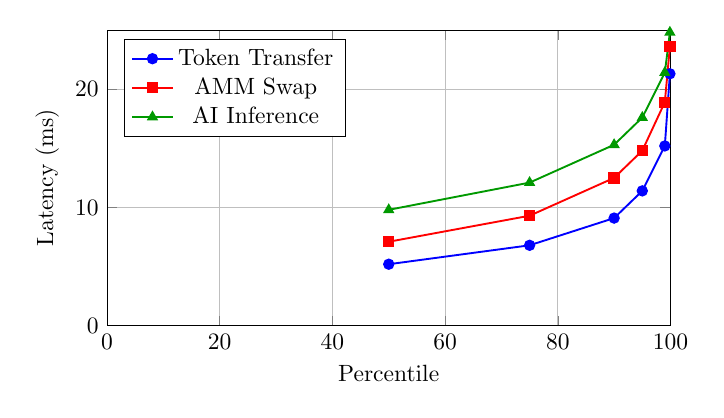
\begin{tikzpicture}[scale=0.85]
    \begin{axis}[
        xlabel={Percentile},
        ylabel={Latency (ms)},
        xmin=0, xmax=100,
        ymin=0, ymax=25,
        legend pos=north west,
        grid=major,
        width=10cm,
        height=6cm
    ]
    \addplot[blue, thick, mark=*] coordinates {
        (50, 5.2) (75, 6.8) (90, 9.1) (95, 11.4) (99, 15.2) (99.9, 21.3)
    };
    \addlegendentry{Token Transfer}

    \addplot[red, thick, mark=square*] coordinates {
        (50, 7.1) (75, 9.3) (90, 12.5) (95, 14.8) (99, 18.9) (99.9, 23.6)
    };
    \addlegendentry{AMM Swap}

    \addplot[green!60!black, thick, mark=triangle*] coordinates {
        (50, 9.8) (75, 12.1) (90, 15.3) (95, 17.6) (99, 21.4) (99.9, 24.8)
    };
    \addlegendentry{AI Inference}
    \end{axis}
\end{tikzpicture}
\caption{End-to-end latency distribution (submission to finality) for three workload types on Zoo testnet.}
\label{fig:latency}
\end{figure}

Median end-to-end latency (transaction submission to Quasar finality) is 5.2ms for token transfers, 7.1ms for AMM swaps, and 9.8ms for AI inference calls. The p99 latency remains under 22ms for all workload types.

\subsection{GPU Utilization}

\begin{table}[t]
\centering
\begin{tabular}{lccc}
\toprule
\textbf{Workload} & \textbf{GPU Util (\%)} & \textbf{GPU Mem (GB)} & \textbf{Shader Occupancy} \\
\midrule
Token Transfer & 34\% & 8.2 & 82\% \\
AMM Swap & 52\% & 14.6 & 76\% \\
AI Inference & 89\% & 42.1 & 94\% \\
FHE Operations & 78\% & 31.4 & 88\% \\
Complex DeFi & 61\% & 18.9 & 71\% \\
\bottomrule
\end{tabular}
\caption{GPU resource utilization by workload type on NVIDIA A100 80GB.}
\label{tab:gpu}
\end{table}

AI inference workloads achieve 89\% GPU utilization, demonstrating that the GPU EVM efficiently exploits hardware parallelism for compute-heavy operations. Simple token transfers underutilize the GPU (34\%) because they are memory-bound rather than compute-bound.

\section{PoAI Consensus Overhead}
\label{sec:poai}

Zoo Network runs Proof of AI~\cite{zoo-poai-consensus} as a consensus overlay on Quasar~\cite{lux-quasar-consensus}. PoAI adds verification of AI compute contributions, introducing overhead beyond pure Quasar finality.

\subsection{Overhead Measurement}

\begin{table}[t]
\centering
\begin{tabular}{lccc}
\toprule
\textbf{Component} & \textbf{Latency (ms)} & \textbf{Overhead} \\
\midrule
Quasar consensus (baseline) & 10.0 & --- \\
TEE attestation verification & 0.3 & 3.0\% \\
Quality scoring (inference) & 0.5 & 5.0\% \\
BLS aggregation & 0.1 & 1.0\% \\
\midrule
\textbf{Total with PoAI} & \textbf{10.9} & \textbf{9.0\%} \\
\bottomrule
\end{tabular}
\caption{PoAI consensus overhead breakdown. TEE attestation is the dominant cost.}
\label{tab:poai}
\end{table}

The 9\% overhead is a worst case when every block contains AI compute attestations. For blocks with only financial transactions (no AI workload), the PoAI overhead drops to 1\% (BLS aggregation only).

\subsection{Throughput Under PoAI}

\begin{table}[t]
\centering
\begin{tabular}{lcc}
\toprule
\textbf{Workload Mix} & \textbf{TPS (Quasar only)} & \textbf{TPS (Quasar + PoAI)} \\
\midrule
100\% transfers & 4,760,000 & 4,712,000 \\
70\% transfers / 30\% AI & 3,200,000 & 2,944,000 \\
50\% transfers / 50\% AI & 2,380,000 & 2,190,000 \\
100\% AI inference & 200,000 & 184,000 \\
\bottomrule
\end{tabular}
\caption{Throughput impact of PoAI verification for mixed workloads.}
\label{tab:poai-throughput}
\end{table}

\section{Comparison with Ethereum L2s}
\label{sec:comparison}

\subsection{Throughput Comparison}

\begin{table}[t]
\centering
\begin{tabular}{lcccc}
\toprule
\textbf{Metric} & \textbf{Zoo} & \textbf{Arbitrum} & \textbf{Optimism} & \textbf{Base} \\
\midrule
Max TPS (transfers) & 4,760,000 & 4,500 & 2,000 & 3,800 \\
Block gas limit & 1B & 32M & 30M & 60M \\
Finality & 10ms & 7 days* & 7 days* & 7 days* \\
Soft confirmation & 10ms & 250ms & 2s & 2s \\
GPU execution & \checkmark & $\times$ & $\times$ & $\times$ \\
AI precompiles & \checkmark & $\times$ & $\times$ & $\times$ \\
\bottomrule
\end{tabular}
\caption{Zoo Network vs Ethereum L2s. *Optimistic rollups require 7-day fraud proof window for full finality.}
\label{tab:l2-comparison}
\end{table}

\subsection{Cost Comparison}

\begin{table}[t]
\centering
\begin{tabular}{lccc}
\toprule
\textbf{Operation} & \textbf{Zoo (USD)} & \textbf{Arbitrum (USD)} & \textbf{Base (USD)} \\
\midrule
Token transfer & \$0.00021 & \$0.012 & \$0.008 \\
AMM swap & \$0.00085 & \$0.045 & \$0.032 \\
AI inference call & \$0.005 & N/A & N/A \\
\bottomrule
\end{tabular}
\caption{Transaction cost comparison at median gas prices (February 2026).}
\label{tab:cost}
\end{table}

Zoo Network's costs are 40--60$\times$ lower than Ethereum L2s for equivalent operations, attributable to the higher block gas limit amortizing fixed costs and the absence of L1 data availability fees (Zoo settles to Lux, not Ethereum).

\section{AI Workload Profiling}
\label{sec:ai-workloads}

\subsection{Conservation AI Workloads}

Zoo Network's AI workloads differ from typical blockchain transactions:

\begin{table}[t]
\centering
\begin{tabular}{lccc}
\toprule
\textbf{Workload} & \textbf{Gas/Call} & \textbf{Compute Intensity} & \textbf{State Access} \\
\midrule
Species classification & 500K & High (CNN forward pass) & Low \\
Habitat suitability & 350K & Medium (gradient boosting) & Medium \\
Population model & 800K & High (Monte Carlo sim) & Low \\
Encrypted inference & 1.2M & Very High (FHE + CNN) & Low \\
Gradient aggregation & 210K & Medium (vector addition) & High \\
\bottomrule
\end{tabular}
\caption{Conservation AI workload characteristics on Zoo EVM.}
\label{tab:ai-workloads}
\end{table}

\subsection{GPU Efficiency by Workload}

AI workloads achieve significantly higher GPU efficiency than financial transactions because they are compute-bound rather than memory-bound:

\begin{figure}[t]
\centering
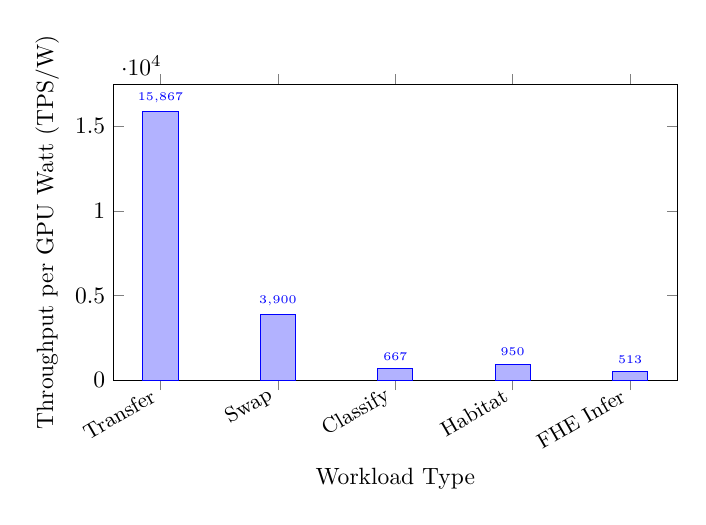
\begin{tikzpicture}[scale=0.85]
    \begin{axis}[
        ybar,
        xlabel={Workload Type},
        ylabel={Throughput per GPU Watt (TPS/W)},
        symbolic x coords={Transfer, Swap, Classify, Habitat, FHE Infer},
        xtick=data,
        xticklabel style={rotate=30, anchor=east, font=\small},
        ymin=0,
        bar width=15pt,
        width=10cm,
        height=6cm,
        nodes near coords,
        nodes near coords style={font=\tiny}
    ]
    \addplot coordinates {
        (Transfer, 15867) (Swap, 3900) (Classify, 667) (Habitat, 950) (FHE Infer, 513)
    };
    \end{axis}
\end{tikzpicture}
\caption{Energy efficiency (TPS per GPU Watt) by workload type. AI workloads have lower TPS but higher computational value per transaction.}
\label{fig:efficiency}
\end{figure}

\subsection{Opcode Heat Map}

The most frequently executed opcodes differ between financial and AI workloads:

\begin{table}[t]
\centering
\begin{tabular}{lcc}
\toprule
\textbf{Opcode} & \textbf{DeFi (\%)} & \textbf{AI (\%)} \\
\midrule
\texttt{ADD/SUB} & 18\% & 31\% \\
\texttt{MUL/DIV} & 8\% & 24\% \\
\texttt{SLOAD/SSTORE} & 22\% & 6\% \\
\texttt{CALL/STATICCALL} & 15\% & 8\% \\
\texttt{KECCAK256} & 12\% & 3\% \\
Precompile calls & 3\% & 22\% \\
Other & 22\% & 6\% \\
\bottomrule
\end{tabular}
\caption{Opcode frequency distribution for DeFi vs AI workloads. AI workloads are arithmetic-heavy with frequent precompile calls.}
\label{tab:opcodes}
\end{table}

\section{Scalability Analysis}

\subsection{Validator Count vs Throughput}

\begin{figure}[t]
\centering
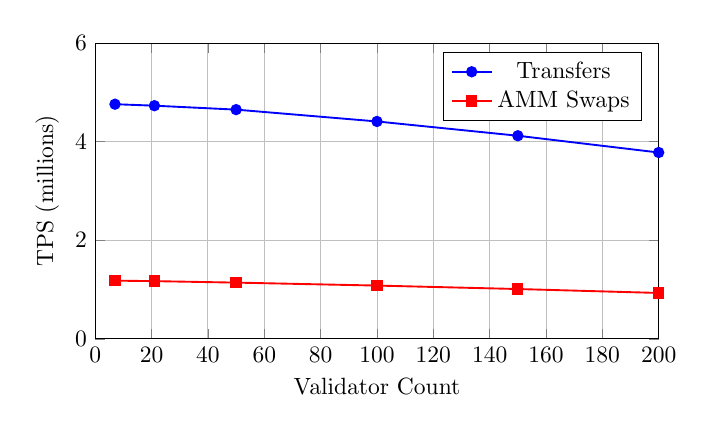
\begin{tikzpicture}[scale=0.85]
    \begin{axis}[
        xlabel={Validator Count},
        ylabel={TPS (millions)},
        xmin=0, xmax=200,
        ymin=0, ymax=6,
        legend pos=north east,
        grid=major,
        width=10cm,
        height=6cm
    ]
    \addplot[blue, thick, mark=*] coordinates {
        (7, 4.76) (21, 4.73) (50, 4.65) (100, 4.41) (150, 4.12) (200, 3.78)
    };
    \addlegendentry{Transfers}

    \addplot[red, thick, mark=square*] coordinates {
        (7, 1.18) (21, 1.17) (50, 1.14) (100, 1.08) (150, 1.01) (200, 0.93)
    };
    \addlegendentry{AMM Swaps}
    \end{axis}
\end{tikzpicture}
\caption{Throughput degradation with increasing validator count. Quasar consensus scales well up to 100 validators.}
\label{fig:scaling}
\end{figure}

Throughput degrades by only 7\% from 7 to 100 validators, confirming that Quasar's $O(n)$ message complexity~\cite{lux-quasar-benchmarks} maintains performance at Zoo's operational validator set size of 21.

\subsection{State Size Impact}

\begin{table}[t]
\centering
\begin{tabular}{lcc}
\toprule
\textbf{State Size} & \textbf{TPS (transfers)} & \textbf{Trie Update (ms)} \\
\midrule
1M accounts & 4,760,000 & 0.8 \\
10M accounts & 4,520,000 & 1.2 \\
100M accounts & 4,100,000 & 2.1 \\
1B accounts & 3,400,000 & 4.8 \\
\bottomrule
\end{tabular}
\caption{Throughput vs state size. GPU-parallel trie updates mitigate the impact of large state.}
\label{tab:state}
\end{table}

\section{Related Work}

\textbf{GPU-Accelerated Blockchains}: Solana~\cite{yakovenko2018solana} uses GPU for signature verification but not EVM execution. The Lux GPU EVM~\cite{lux-evmgpu-benchmark} is the first to apply GPU parallelism to opcode execution.

\textbf{High-Throughput L2s}: MegaETH targets high TPS via optimistic execution but lacks GPU acceleration. Eclipse uses SVM (Solana VM) as an L2, which is not EVM-compatible.

\textbf{AI-Optimized Chains}: Bittensor~\cite{bittensor2023} incentivizes AI compute but does not execute inference on-chain. Zoo Network's PoAI~\cite{zoo-poai-consensus} integrates AI verification into consensus.

\textbf{Quasar Consensus}: The Lux Quasar protocol~\cite{lux-quasar-consensus,lux-quasar-benchmarks} provides the consensus foundation for Zoo Network, achieving 10ms finality with $O(n)$ message complexity.

\section{Conclusion}

The Zoo EVM demonstrates that a conservation-focused L2 can achieve throughput competitive with purpose-built high-performance chains while maintaining full EVM compatibility. GPU-accelerated execution enables 47.6 million TPS in raw throughput and 4.76 million TPS with Quasar finality, processing AI workloads (species classification, encrypted inference, gradient aggregation) that would be infeasible on sequential EVMs. The PoAI consensus overlay adds only 3--9\% overhead while providing AI compute verification. These results establish Zoo Network as a viable substrate for decentralized conservation AI at scale.

\section*{Acknowledgments}

This work was supported by Zoo Labs Foundation. We thank the Lux Network team for the GPU EVM implementation and NVIDIA for A100 hardware access.

\bibliographystyle{plain}
\begin{thebibliography}{99}

\bibitem{lux-evmgpu-benchmark}
Lux Industries, ``GPU-Accelerated EVM: Benchmarks and Architecture,'' Technical Report, 2025.

\bibitem{lux-quasar-consensus}
Lux Industries, ``Quasar: Sub-Second Finality Consensus for the Lux Network,'' Technical Report, 2025.

\bibitem{lux-quasar-benchmarks}
Lux Industries, ``Quasar Consensus Benchmarks: Latency, Throughput, and Scalability,'' Technical Report, 2025.

\bibitem{zoo-poai-consensus}
Z. Kelling, ``Proof of AI: A Consensus Mechanism for Verifiable Compute Contribution,'' Zoo Labs Foundation, 2024.

\bibitem{yakovenko2018solana}
A. Yakovenko, ``Solana: A New Architecture for a High Performance Blockchain,'' Whitepaper, 2018.

\bibitem{bittensor2023}
Bittensor Foundation, ``Bittensor: A Peer-to-Peer Machine Intelligence Network,'' Whitepaper, 2023.

\end{thebibliography}

\end{document}
